\documentclass[tikz]{standalone}
\usepackage{pgfplots}
\pgfplotsset{compat=1.18}
\definecolor{bgdark}{HTML}{171D2B}
\definecolor{aksen}{HTML}{F7B538}
\begin{document}
\pagecolor{bgdark}
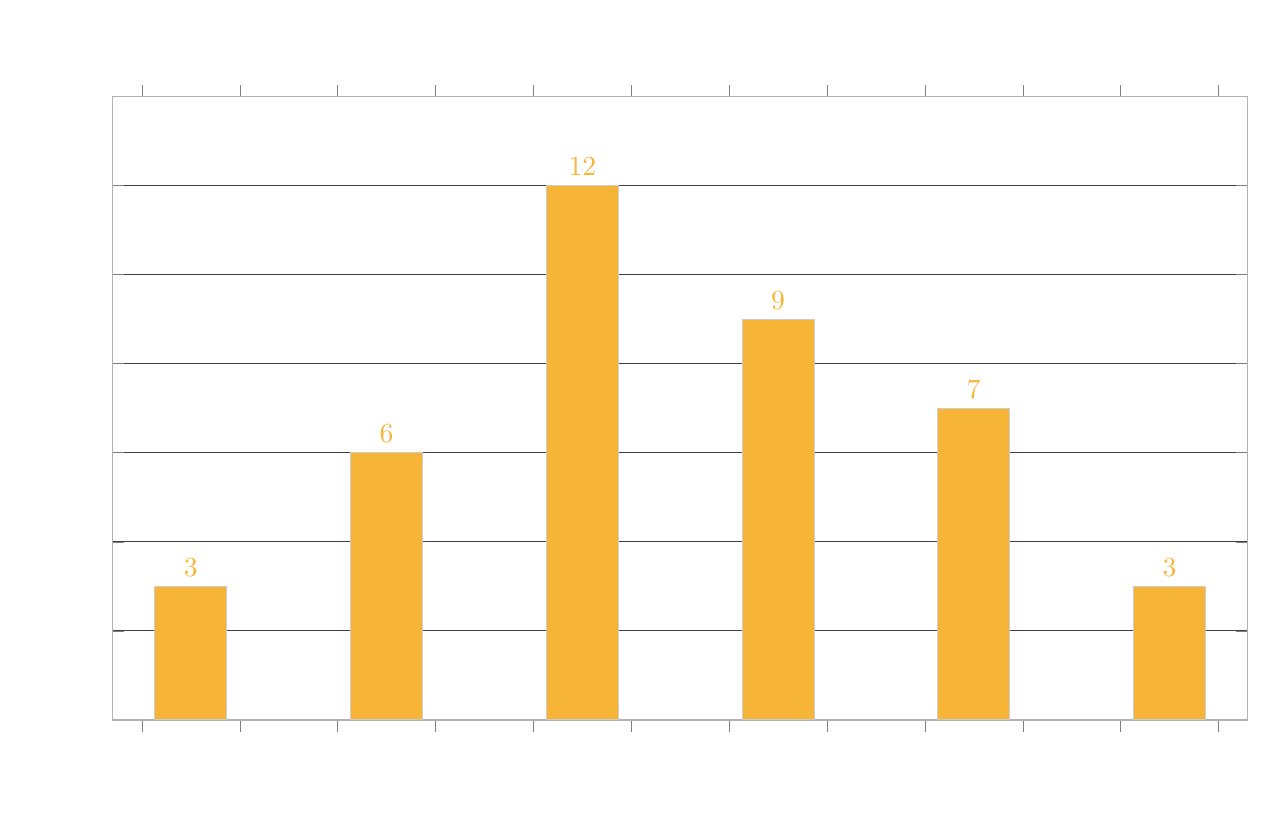
\begin{tikzpicture}[text=white,font=\sffamily]
\begin{axis}[
  width=16cm, height=9.5cm,
  axis line style={white!70!black},
  x tick label style={/pgf/number format/1000 sep=},
  title={Nilai Ulangan Matematika (40 siswa)},
  title style={font=\bfseries\large},
  xlabel={Nilai}, ylabel={Frekuensi},
  ybar=2pt, bar width=26pt,
  ymin=0, ymax=14,
  enlarge x limits=0.08,
  ymajorgrids=true, grid style={white!25!black},
  every node near coord/.append style={color=aksen,font=\bfseries},
  nodes near coords,
]
\addplot[fill=aksen, draw=white!80!black] coordinates
{(47.5,3) (57.5,6) (67.5,12) (77.5,9) (87.5,7) (97.5,3)};
\end{axis}
\end{tikzpicture}
\end{document}
